\documentclass[aspectratio=169]{beamer}

\mode<presentation>
\usetheme{Boadilla}
\definecolor{redback}{RGB}{140,0,0}
\definecolor{blue}{RGB}{30,90,205}
\definecolor{red}{RGB}{213,94,0}
\definecolor{green}{RGB}{0,128,0}
\setbeamercolor{title}{fg=redback}
\setbeamercolor{frametitle}{fg=redback}
\setbeamercolor{block title}{bg=redback, fg=white}
\setbeamercolor{block body}{bg=white}
\setbeamercolor{structure}{fg=redback}
\setbeamercolor{item projected}{fg=white}
\setbeamercolor{item}{fg=redback}
\setbeamercolor{subitem}{fg=redback}
\setbeamercolor{section in toc}{fg=redback}
\setbeamercolor{description item}{fg=redback}
\setbeamercolor{caption name}{fg=redback}
\setbeamercolor{button}{bg=redback, fg=white}
\setbeamercolor{caption name}{fg=redback}
\usepackage{graphics}
\usepackage{tikz}
\usepackage{amsmath}
\usepackage{bbm}
\usetikzlibrary{decorations.pathreplacing}
\usepackage{geometry}
\usepackage{booktabs}
\usepackage{multirow, makecell}
\usepackage{float}
\usepackage{fancyvrb}
\usepackage{kotex}
\usepackage{caption}
\usepackage{subcaption}
\usepackage{adjustbox}
\usepackage{hyperref}
\usepackage{threeparttable}
\usepackage[scaled=0.92]{helvet}
\usepackage[default]{lato} %If I want a twist
\newenvironment{wideitemize}{\itemize\addtolength{\itemsep}{10pt}}{\enditemize}
\newenvironment{wideenumerate}{\enumerate\addtolength{\itemsep}{10pt}}{\endenumerate}
\newenvironment{widedescription}{\description\addtolength{\itemsep}{10pt}}{\enddescription}
\hypersetup{
colorlinks=true,
linkcolor=redback,
filecolor=green, 
urlcolor=blue,
}
\beamertemplatenavigationsymbolsempty
\setbeamercolor{author in head/foot}{bg=white, fg=redback}
\setbeamercolor{title in head/foot}{bg=white, fg=redback}
\setbeamercolor{date in head/foot}{bg=white, fg=redback}
\setbeamercolor{section in head/foot}{bg=white, fg=redback}
\setbeamercolor{page number in head/foot}{bg=white, fg=redback}
\setbeamercolor{headline}{bg=redback}
\setbeamertemplate{footline}{
    \leavevmode%
    \hbox{%
        \begin{beamercolorbox}[wd=.333333\paperwidth,ht=2.25ex,dp=1ex,center]{date in head/foot}%
            \usebeamerfont{date in head/foot}\insertshortdate
        \end{beamercolorbox}%
        \begin{beamercolorbox}[wd=.444444\paperwidth,ht=2.25ex,dp=1ex,center]{title in head/foot}%
            \usebeamerfont{title in head/foot}\insertshorttitle
        \end{beamercolorbox}%
        \begin{beamercolorbox}[wd=.222222\paperwidth,ht=2.25ex,dp=1ex,center]{page number in head/foot}%
            \usebeamerfont{page number in head/foot} \insertframenumber{} / \inserttotalframenumber
        \end{beamercolorbox}}%
        \vskip0pt%
    }

\setbeamertemplate{section in toc}[sections numbered]
\setbeamertemplate{subsection in toc}{\leavevmode\leftskip=3em\rlap{\hskip-1.75em\inserttocsectionnumber.\inserttocsubsectionnumber}\inserttocsubsection\par}
\setbeamerfont{subsection in toc}{size=\footnotesize}

\newenvironment{transitionframe}{\setbeamercolor{background canvas}{bg=redback}\setbeamertemplate{footline}{} \begin{frame}}{\end{frame}}
\newcommand{\ROM}[1]
    {\MakeUppercase{\romannumeral #1}}
    \DeclareMathOperator*{\plim}{plim}
\makeatletter
\let\@@magyar@captionfix\relax
\makeatother


\title[Recitation 13 (Intro to Econometrics \ROM{2})]{Recitation 13: Random forests and artificial neural networks} % Change this regularly
\author[]{Seung-hun Lee }
\institute[]{Columbia University \\ Introduction to Econometrics \ROM{2} Recitation}

\date[May 2nd, 2022]{May 2nd, 2022}

\begin{document}
\begin{frame}
\titlepage
\end{frame}


%%% Color slides for section headers: Use for colloquium version (The ones bewteen \iffals and \fi)

\begin{transitionframe}
  \begin{center}
         { \Huge \textcolor{white}{Random forest}}
       \end{center}
\end{transitionframe}

\begin{frame}
\frametitle{Classical random forests: Classification and regression trees}
\begin{itemize}
\item We have an IID data $(y_i,x_i)$ for $i\in\{1,...,n\}$
\item Decision trees represent classification and regression problems using nonlinear basis functions (indicators of categories or cutoff)
\begin{itemize}
\item Branch: Path from one node to other
\item Split: Process of dividing a sample based on a criterion specified at a node; creates two branches per non-terminal nodes
\item Depth: Number of stages with splits
\item Leaves: Output; or nodes on the last stage
\item Pruning: Reducing the size of the tree (steps or fewer splits)
\end{itemize} 
\item The goal is to find an algorithm that best predicts out-sample properties
\end{itemize}
\end{frame}

\begin{frame}
\frametitle{CART uses recursive greedy algorithm}
\begin{itemize}
\item Recursive in that there are repeated nodes with partitioning of two-way splits
\begin{itemize}
\item Select a variable $x_k$ and threshold/class that allows each split outcome to be as different as possible (between variance and information gain)
\item Between variance: Variation between each group mean to overall mean, $R^2$ of
\[
y=\beta\mathbb{I}(x_k>t)+u
\]
\item Information gain: For a potential split $S=S_1\cup S_2$ 
\[
IG = L(S)-\left[\frac{|S_1|}{|S|}L(S_1)+\frac{|S_2|}{|S|}L(S_2)\right], \ \ L(C)=-\sum_{j=1}^J f_j \log{f_j}
\]
i.e. splits $S_1$ and $S_2$ that has lower combined entropies (leading to high IG)
\end{itemize}
\item Greedy in that at each non-terminal node, the best test selected is only locally optimal
\begin{itemize}
\item No look-forward
\item Due to NP-hardness of the optimal tree problem, this is cheaper
\end{itemize}
\end{itemize}
\end{frame}


\begin{frame}
\frametitle{Finding the best CART is not easy}
\begin{itemize}
\item Selection of hyperparameters (parameters whose value is used to control the learning process such as split criterion, stopping criteria)
\begin{itemize}
\item Can lead to overfitting and bad out-sample predictions if improperly selected
\end{itemize}
\item Pruning: Making the trees more compact by eliminating some splits
\begin{itemize}
\item Cross-validation is used
\end{itemize}
\item Greedy algorithm: Decision tree may not be stable and the most optimal possible, especially when the top node is incorrectly selected
\end{itemize}
\end{frame}

\begin{frame}
\frametitle{Bootstrap AGGregatING, or Bagging}
\begin{itemize}
\item Like ensemble method, it averages from multiple decision trees to enhance stability and accuracy of prediction, classification, and regression
\item By averaging, bagging protects from overfitting the data and prevents instability
\item The procedure is very similar to that of bootstrapping. They are as follows
\begin{itemize}
\item[1.] Bootstrap: Let's have a sufficiently large $B$ resamples with replacement. In each resampling step, we fit a tree.
\item[2.] Aggregation: We average the predictions of the $B$ trees to predict $y$ given $x$. 
\end{itemize}
\item Predictive capability: Are the predictions less dispersed? Then this is good prediction
\end{itemize}
\end{frame}


\begin{frame}
\frametitle{Random Forest}
\begin{itemize}
\item Averaging multiple deep decision trees, trained on different parts of the same training data set
\item  Unlike bagging, random forests choose splits from a smaller number of randomly selected covariates at each step of the tree construction (feature bagging)
\begin{itemize}
\item With $k$ available features, $\sqrt{k}$ is used in classification and $\max\{k/3,5\}$ in regression
\end{itemize}
\item Less correlation among trees compared to earlier methods (variety of top splits)
\item Less overfitting and more stability
\begin{itemize}
\item Variable with huge decline in split-criterion (out-of-bag-error from permutation over $B$ trees) can be considered important
\end{itemize}
\item Key problem is loss of interpretability (black-box procedure in selection of covariates)
\end{itemize}
\end{frame}

\begin{frame}
\frametitle{Causal forest (Wagner, Athey 2018)}
\begin{itemize}
\item Random forest to estimate treatment effect (under CIA)
\item We first estimate the propensity score $\hat{p}_i$ and transform $y_i$ into
\[
\hat{y}_i = \frac{D_i-\hat{p}_i}{\hat{p}_i(1-\hat{p}_i)}y_i
\]
which is an IPW formula
\item By taking the expected value of $\hat{y}_i$ we get
\[
\widehat{TE}(x)=E[\hat{y}_i|x]
\]
\item We then do `honest' inference (defined in the paper) by estimating on a subsample that is different from the training and test subsamples (double-sample trees)
\item We can also do normal inference
\end{itemize}
\end{frame}

\begin{frame}
\frametitle{Local linear forest (Friedberg, Tibshirani, Athey, Wagner 2020)}
\begin{itemize}
\item Random forests are used to generate weights that can serve as a kernel for a local linear regression and estimates for the conditional mean function
\item Think of random forests as adaptive weight generators
\[
\hat{m}(x_0)=\frac{1}{B}\sum_{i=1}^n \sum_{b=1}^By_i \frac{\mathbb{I}[X_i\in L_b(x_0)]}{|L_b(x_0)|}=\sum_{i=1}^n y_i \underbrace{\frac{1}{B}\sum_{b=1}^B\frac{\mathbb{I}[X_i\in L_b(x_0)]}{|L_b(x_0)|}}_{\alpha_i(x_0)}
\]
\item $L_b(x_0)$ represents the leaf at $b$'th tree, $|\cdot|$ indicates the size of the leaves. 
\item $\alpha_i(x_0)$ is the fraction of trees in which an observation appears in the same leaf as the target value of the covariate vector
\end{itemize}
\end{frame}

\begin{frame}
\frametitle{Local linear forest (Friedberg, Tibshirani, Athey, Wagner 2020)}
\begin{itemize}
\item Local linear forests solve the weighted least problem below with penalty term using the weights defined above
\[
\begin{pmatrix} \hat{m}(x_0) \\ \hat{\theta}(x_0) \end{pmatrix} = \arg\min_{m,\theta}\left[ \sum_{i=1}^n \alpha_i(x_0) (y_i-m(x_0)-(x-x_0)\theta(x_0))^2 +\lambda ||\theta(x_0)||^2\right]
\]
\item Performs better when smooth, strong signals are present (random forests don't do so well in this case)
\item Also overcomes curse of dimensionality
\end{itemize}
\end{frame}

\begin{frame}
\frametitle{Gradient-boosted trees}
\begin{itemize}
\item Improve the performance of weak learners by boosting the weight of observations they misspecify
\item Start with a loss function $\min \sum_{i=1}^n L(y_i,\hat{y}_i), \ \text{say, } (y_i-\hat{y}_i)^2$
\item $v(x,S)$: Average value of $y$ in the leaf that contains $x$ in a shallow tree with splits $S$
\item Then we proceed in these steps
\begin{itemize}
\item[1.] Begin with an initial prediction: $\hat{y}_i^{(0)}=E[y_i]$
\item[2.] For each iteration $b\in\{1,...,B\}$, we choose split $S_b$ in the tree of depth $d$ to minimize
\[
\sum_{i=1}^n L(y_i, \hat{y}_i^{(b-1)}+v(x_i,S) )
\]
and update our prediction $\hat{y}_i^{(b)}= \hat{y}_i^{(b-1)}+\epsilon v(x_i,S_b)$. Note that $\epsilon$ is the learning rate and is not $\epsilon=1$, which would mean updating the prediction by the exact value and risk overshooting
\end{itemize}
\end{itemize}
\end{frame}


\begin{frame}
\frametitle{Other ways to do gradient-boosted trees}
\begin{itemize}
\item We can also tune the model by including a complexity penalty in the loss function. So we minimize 
\[
\sum_{i=1}^n L(y_i, \hat{y}_i^{(b-1)}+v(x_i,S) ) + C(S)
\]
\item XGBoost: Extreme gradient-boosting, increases the speed of the procedure using quadratic loss and complexity penalty functions
\[
\sum_{i=1}^n (G_iv(x_i, S)+\frac{1}{2} H_i v(x_i,S)^2)+ \gamma K + \frac{\lambda}{2}\sum_{k=1}^K v_k^2
\]
where $G_i$ and $H_i$ are each the first and second derivatives of the $L(y_i. \hat{y}_i)$ w.r.t $\hat{y}_i$ at $(y_i, \hat{y}_i^{(b-1)})$, $K$ is the number of leaves, and $v_k$ is the predictor on leaf $k$
\item Tuning and some hyperparameters still need to be determined
\end{itemize}
\end{frame}

\begin{transitionframe}
  \begin{center}
         { \Huge \textcolor{white}{Artificial neural networks}}
       \end{center}
\end{transitionframe}


\begin{frame}
\frametitle{Architecture of artificial neural networks}
\begin{figure}[H]
\centering
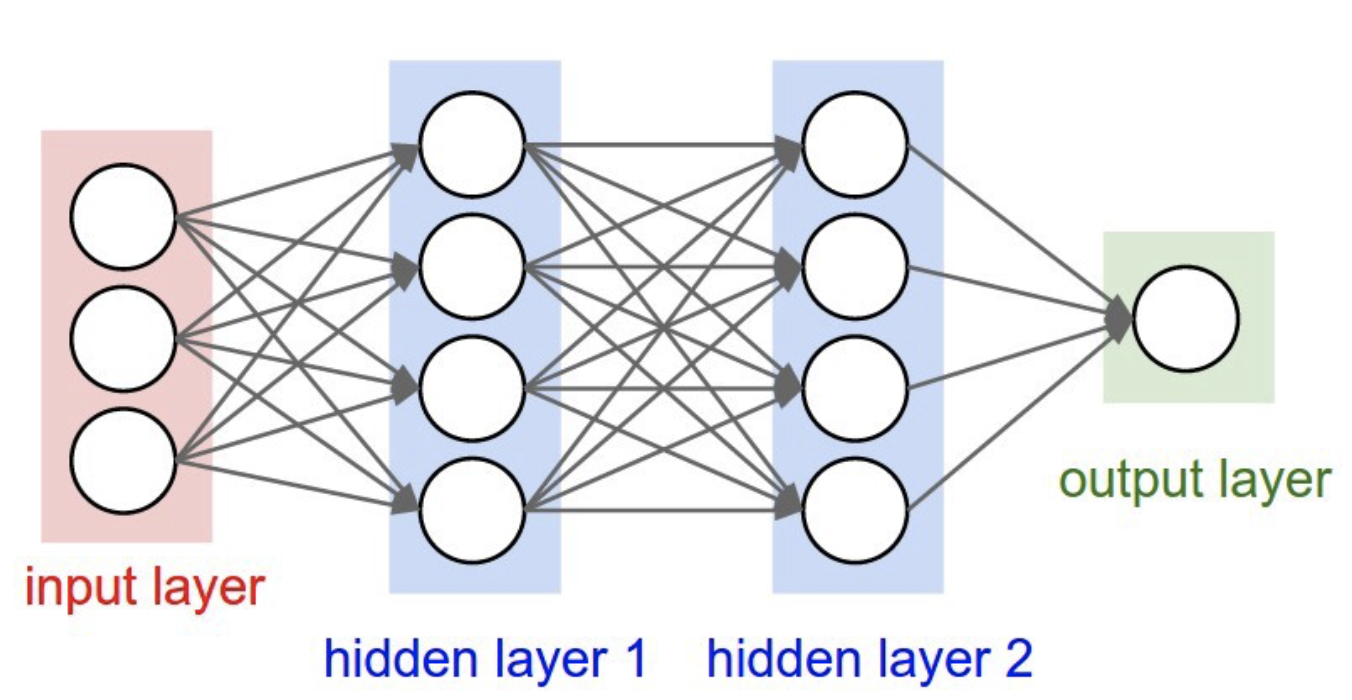
\includegraphics[width=0.8\textwidth, keepaspectratio]{neuralnetwork.png}
\end{figure}
\end{frame}

\begin{frame}
\frametitle{Architecture of artificial neural networks}
\begin{itemize}
\item Input layers have covariates $x_m$
\item Lines between layers have weights $w$
\item Each direction represents signal $\sigma(\cdot)$, known as activation function
\begin{itemize}
\item A sigmoid (logit)
\item Multinomial logit (softmax)
\item Rectified linear unit (ReLU, $\sigma(t)=\max\{0,t\}$)
\end{itemize}
\end{itemize}
\end{frame}

\begin{frame}
\frametitle{Single layer perceptions: Setup and forward pass}
\begin{itemize}
\item $M$ neurons in input, $L$ nodes in hidden layer
\item Input neurons are denoted $x_1,...,x_M$ have weights $w_{1lm},\ m\in\{1,...,M\},\ l\in\{1,...,L\}$, and emit $\sigma(\sum_{m} w_{1lm}x_m)$ to a hidden layer $l$
\item Hidden layer has weight for each node, $w_{2l}$, used to combine inputs from previous nodes to generate a prediction for the output node $\hat{y} = g\left(\sum_l w_{2l}\sigma(\sum_{m} w_{1lm}x_m)\right)$
\item Epoch: One forward pass + backward pass
\item Forward pass:  Given loss function $L(y,\hat{y}(\theta))$ and an initial value $\theta=(w_1, w_2)$, compute
\[
z_{il}=\sigma(w_{1l}'x_i)
\]
and then the output can be produed as
\small{\[
\hat{y}_i(\theta) = w_2'z_i = \sum_l w_{2l}\sigma\left(\sum_{m} w_{1lm}x_{im}\right)
\] }\normalsize
\end{itemize}
\end{frame}

\begin{frame}
\frametitle{Single layer perceptions: Backward pass}
\begin{itemize}
\item Compute the components of the loss functions, then take gradients with respect to elements in $\theta$, and do approximate Newton iteration (e.g. Minibatch gradient descent)
\[
\theta^{(s+1)}=\theta^{(s)}-\epsilon_s\frac{\partial L}{\partial \theta}(\theta^{(s)})
\]
\item $\epsilon_s$ is the learning rate which ideally should goes to 0
\item Backpropagation: An automated differentiation and application of chain rule to identify gradients used to update the values of the weights
\end{itemize}
\end{frame}

\begin{frame}
\frametitle{Deep learning: Multiple hidden layers}
\begin{itemize}
\item Many (hyper)parameters, activation functions to choose
\item We have $p$ covariates, $K$ outputs, $D$ hidden layers, and $M$ nodes per layer ($p, K$ given)
\item  In total, we have $pM + (D-1)M^2 + kM$ parameters (or weights) to work with
\item Optimal $D$ and $M$? It is known that deep artificial neural networks are preferable to wider ones
\begin{itemize}
\item Small $D$ does not fit well, large $D$ induces less overfitting problem especially if there are many small weights (also, we gain on expressiveness)
\item Incorporating penalty term $\lambda ||\theta||_q^q$ helps too
\end{itemize}
\item Dropout: Randomly eliminates some links and thins the neural networks, which is then retrained and tested/compared with all the eliminated units brought back in
\begin{itemize}
\item Realistic alternative to cross-validation
\end{itemize}
\end{itemize}
\end{frame}

\begin{frame}
\frametitle{Double machine learning debiasing techniques}
\begin{itemize}
\item ATE under CIA
\[
y_ i = \mu(X_i, D_i)+\epsilon_i(D_i), \ D_i=\mathbb{I}(u_i<p(X_i)), \ \ (\epsilon(0), \epsilon(1))\perp\!\!\perp u|X
\]
\item Use ML to estimate the $p(X_i)$ and $\mu(X_i, D_i)$ and obtain IPW ATE
\item Debiasing? $p(X_i)$ and $\mu$ are nuisance parameters whose errors affect TE estimates
\item Decouple the TE from the $p(X_i)$ and $\mu$ using Neyman orthogonalization (block-diagonalize the (Fisher) information matrix) - ML method involved
\begin{itemize}
\item Split data to $K$ folds, and leave one out
\item Estimate $\hat{p}_k=\Pr(D=1|X)$ using LASSO or other ML methods
\item Take the Neyman-orthogonalized combination of the estimates of $p(X_i)$ and $\mu$
\item If functions are smooth, estimates have standard asymptotics and we can do standard tests afterwards
\end{itemize}
\end{itemize}
\end{frame}
%%%%%%%%%%%
\end{document}
